\pagestyle{empty}
\cleardoublepage
\pagestyle{fancy}

\chapter{Apresentação e análise dos resultados}\label{chap:resultado}
% Dias de coleta: select distinct dt_visita from imovel order by 1
% Total de registros: select count(id) from imovel
% Imoveis no Rio: select count(id) from vw_imovel_rio

Em agosto e outubro de 2014 foram coletados 91.091 registros de anúncios de vendas de apartamento do tipo padrão do site ZAP Imóveis. Destes, 58.698 anúncios contém informações de localização geográfica, latitude e longitude. Em seguida, utilizando um filtro espacial para identificar aqueles cujas coordenadas geográficas estão contidos no município do Rio de Janeiro, restaram 58.353.

Teste de SVG

\begin{figure}
\centering
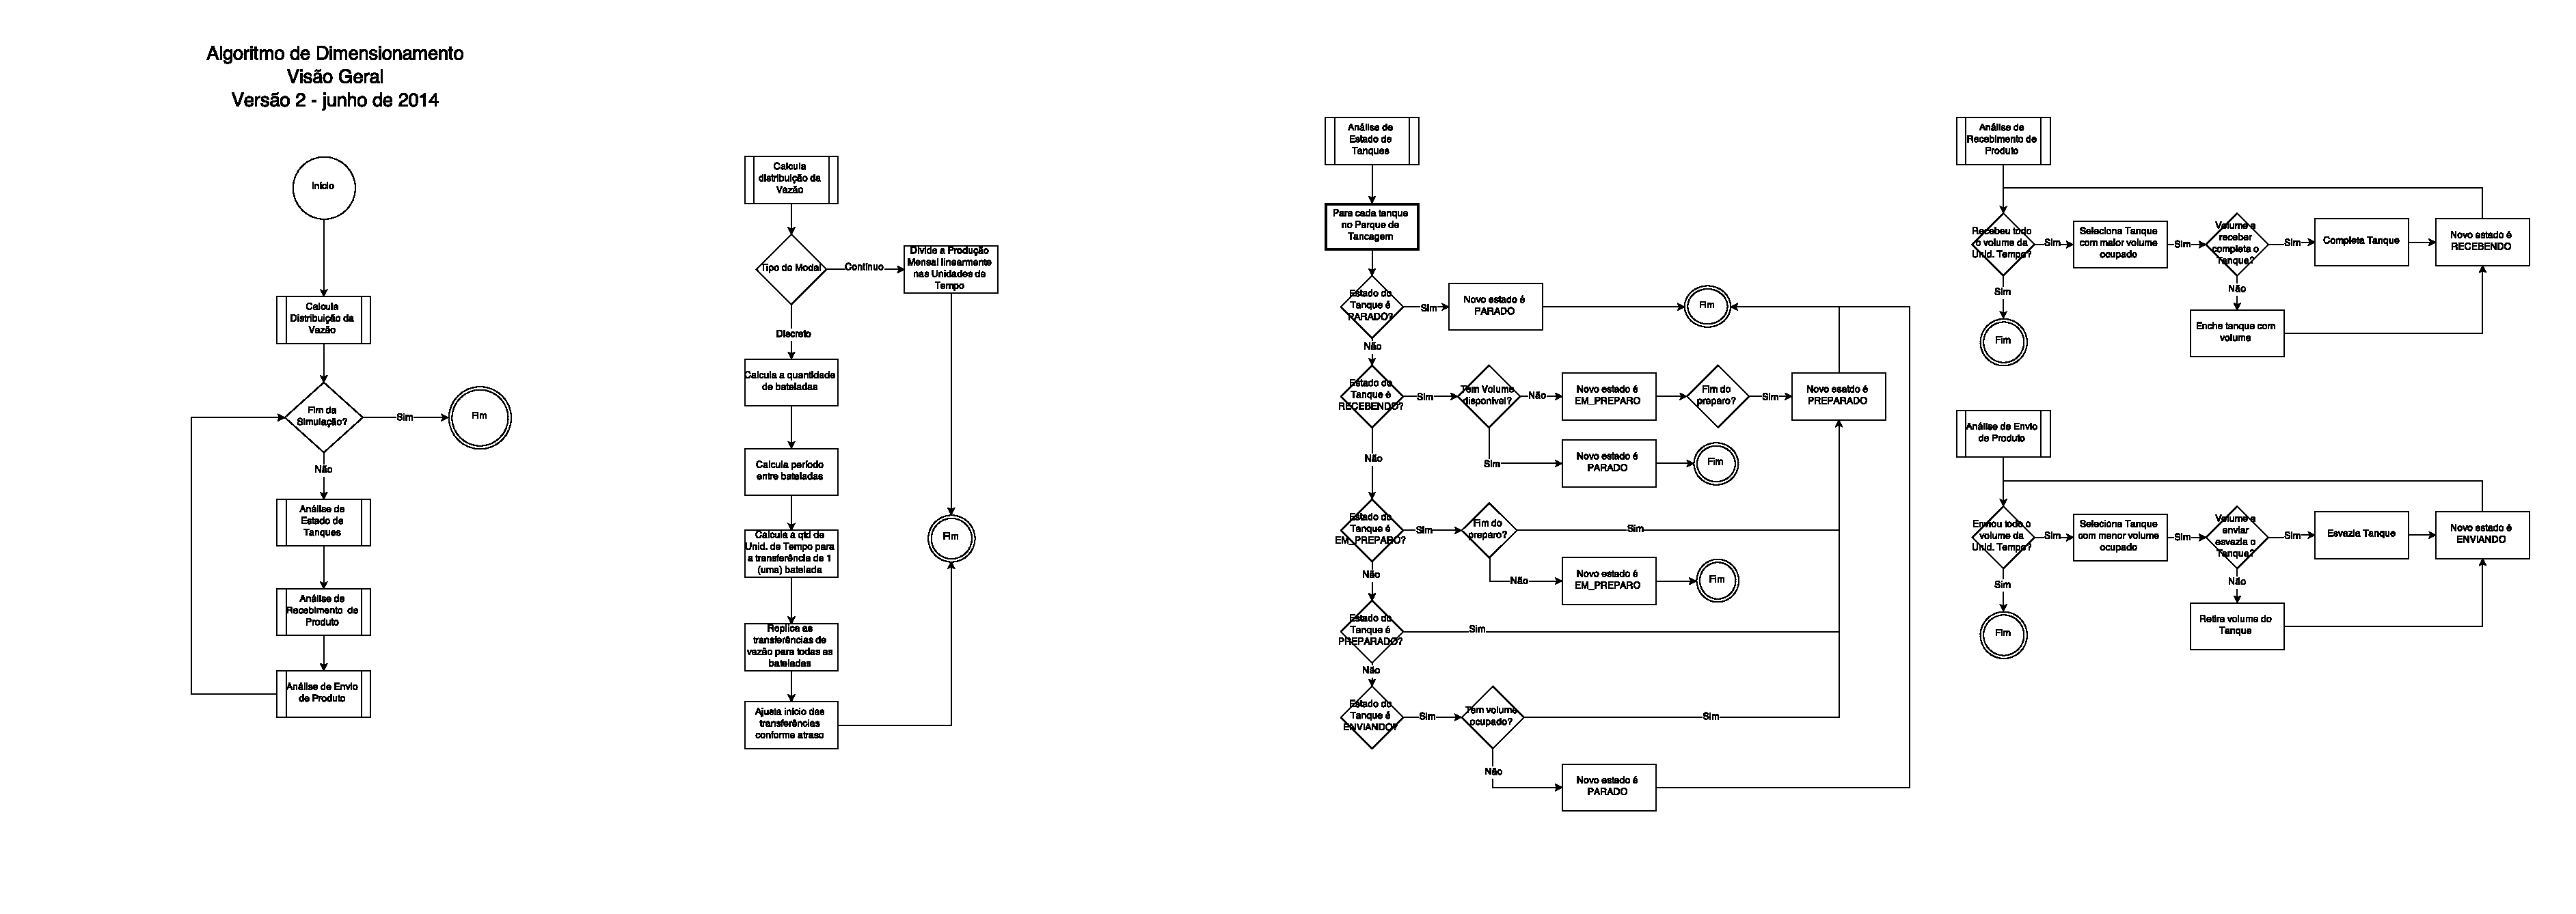
\includegraphics[width=0.7\linewidth]{img/sdtv2}
\caption{}
\label{fig:SDT-DimensionamentoTancagem-v2}
\end{figure}



Após localização espacial usando as coordenadas dos anúncios, alguns bairros destacam-se por não ter nenhum anúncio:

% Bairros sem anúncio: select nome from bairro where nome not in (select distinct bairro_g from vw_imovel)

\begin{table}[htp]
	\begin{center}
		\begin{tabular}{c}
		\toprule
			\textbf{Bairro}\\ \midrule			
			Acari\\
			Engenheiro Leal\\
			Gericinó\\
			Grumari\\
			Mangueira\\
			Paquetá\\
			Parque Colúmbia\\
			Saúde\\
		\bottomrule
		\end{tabular}
	\end{center}
	\caption{Bairros sem imóveis anunciados.}
	\label{tbl_bairros_sem_imovel}
\end{table}

Em uma primeira análise, apresentamos o mapa temático abaixo, identificando os bairros pela média do $m^2$, para todos os imóveis anunciados.

